
	\section{Кристалличность полимеров}


\subsection{Степень кристалличности}
	
	\begin{wrapfigure}{r}{0.5\textwidth} 
\vspace{-20pt}
  \begin{center}
    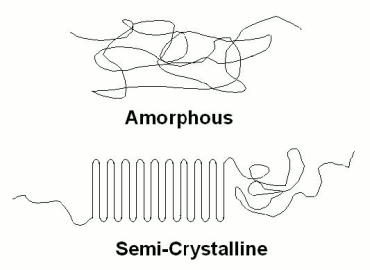
\includegraphics[width=0.4\textwidth]{fig/crystal-1.png}
    \caption{Как цепочки складываются в ламели}
    \label{fig:crystal-1}
  \end{center}
  \vspace{-20pt}
  \vspace{1pt}
\end{wrapfigure}
	
	
	\begin{wrapfigure}{r}{0.5\textwidth} 
\vspace{-20pt}
  \begin{center}
    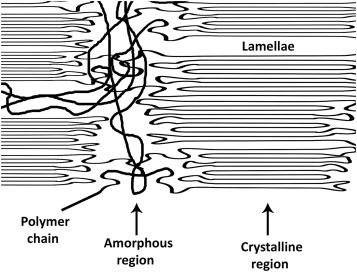
\includegraphics[width=0.4\textwidth]{fig/crystal-2.jpg}
    \caption{К определению кристалличности полимеров}
    \label{fig:crystal-2}
  \end{center}
  \vspace{-20pt}
  \vspace{1pt}
\end{wrapfigure}	
	
\subsection{Кристаллические структуры}

\begin{figure}
    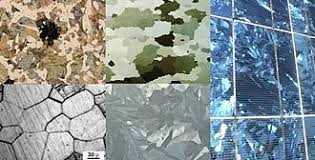
\includegraphics[width=\textwidth]{fig/crystallites.jpg}
    \caption{Типы кристаллитов}
    \label{fig:crystallites}
\end{figure}


	частичность
	
	фазы, кристаллиты
	
\subsection{Полиэфиримиды ряда R-BAPB }
структура

Что следует из первичной структуры, термостойкость, особенности, пригодность для СЛС, перспективность

Данные по композитным добавкам

характеристики - все что измерили в ИВС

Что еще нужно выясеить

		
	\begin{figure}
	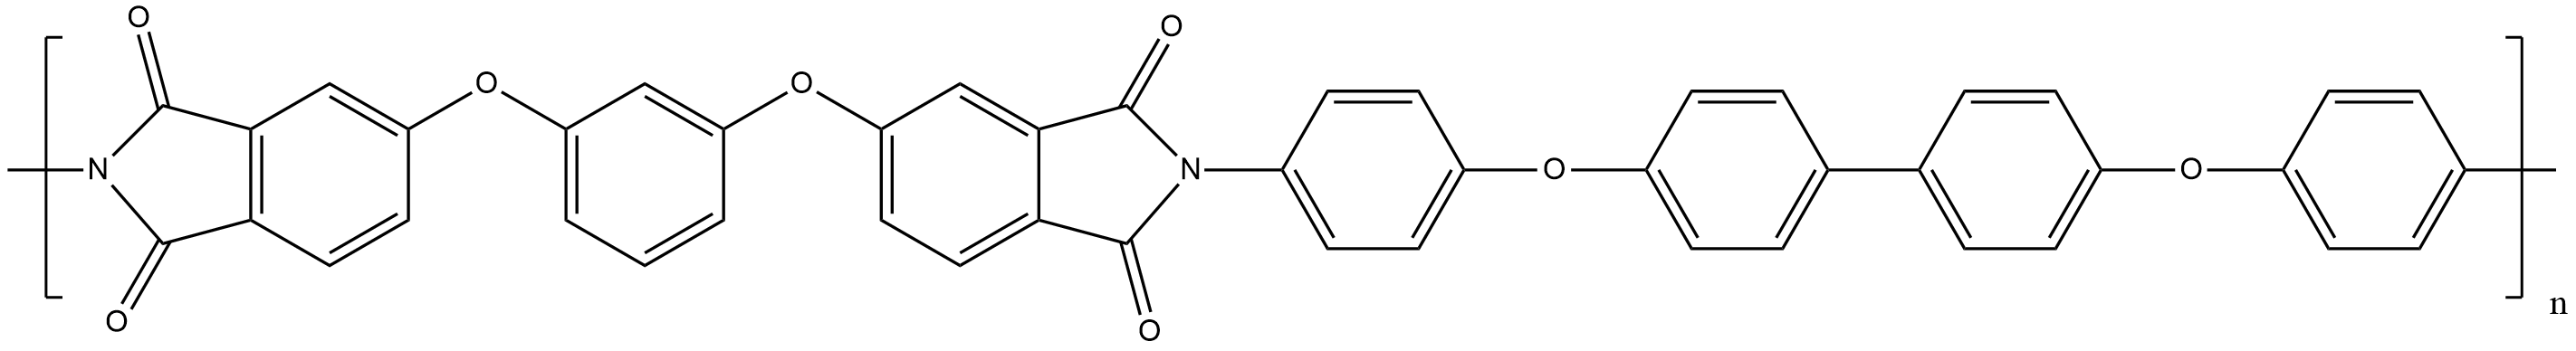
\includegraphics[width=\textwidth]{fig/formula.png}
	\end{figure}
	
	\section{Модель процесса спекания}
	
	\section{Дифракция}
	когерентные источники, йоу!
	
	эффекты от аморфной части
	
	
    \section{Что известно про imaging}
    в теории
    
    гаусс,войт, интегралы
	